\section{A reproducibility crisis}
\includegraphics[page=4,scale=0.6]{01_OS_and_FAIR_intro.pdf}
\includegraphics[page=5,scale=0.6]{01_OS_and_FAIR_intro.pdf}
\includegraphics[page=6,scale=0.6]{01_OS_and_FAIR_intro.pdf}
\includegraphics[page=7,scale=0.6]{01_OS_and_FAIR_intro.pdf}

\section{Open science and FAIR}
\includegraphics[page=10,scale=0.6]{01_OS_and_FAIR_intro.pdf}
\includegraphics[page=11,scale=0.6]{01_OS_and_FAIR_intro.pdf}
\includegraphics[page=13,scale=0.6]{01_OS_and_FAIR_intro.pdf}

\begin{frame}{FAIR session with AuBi}
%\begin{block}{\textbf{F}easibility\textbf{A}ccessibility\textbf{I}nteroperability\textbf{R}eproducibility}
%\begin{itemize}
%\item Render a reproducible work in bioinformatic
%\item Introduction to the FAIR concepts
%\item FAIR training since 2019
%\item Publication related \url{https://jose.theoj.org/papers/10.21105/jose.00068}
%\end{itemize}
%\end{block}

\begin{block}{Objectives}<1->
\begin{itemize}
\item Discover FAIR practices
\item Discover tools for best practices
\item Use tool and best practices in practice sessions
\item 5 sessions for courses and practices
\end{itemize}
\end{block}

\begin{block}{The activity}<2->
\begin{itemize}
\item 5 sessions for courses and practice
\item First session in November 2022
\end{itemize}
\end{block}
\end{frame}

\section{Training content}
\begin{frame}
\begin{block}{Contents}
\begin{itemize}
\item<1-> Introduction to FAIR practices
\item<2-> Code control using Git \faGit* 
	\begin{itemize}[<2->]
	\item Git environment
	\item Gitlab and Github \faGithub \faGitlab
	\end{itemize}
\item<3-> Encapsulation process
	\begin{itemize}[<3->]
	\item Conda environment and packages use 
\includegraphics[scale=0.07]{images/conda_logo.pdf}
	\item Containers as docker \& singularity \faDocker 
	\item Reproducible workflow using snakemake 	
\includegraphics[scale=0.05]{images/snakemake_logo.png}
	\end{itemize}
\item<4-> Literate programming and documentation
	\begin{itemize}[<4->]
	\item Markdown syntax \faMarkdown
	\item Rmarkdown for R \faRProject 
	\item Jupyterlab for Python \faPython
	\end{itemize}
\end{itemize}
\end{block}

\end{frame}

